\section{Initial Experiments}\label{sect:experiments}



In this section, we conduct an initial evaluation of Hogwild! Inference under different conditions. We run our main evaluations with the \textbf{QwQ-32B} model\footnote[7]{\url{https://huggingface.co/Qwen/QwQ-32B}} and consider two evaluation setups: simple synthetic tasks that require minimal communication and a more challenging set of reasoning problems that require more complex collaboration patterns.

\paragraph{Sanity checks with synthetic tasks:} 
Before we try our approach on more challenging tasks, we test if Hogwild!\! Inference is capable of basic collaboration.
For this purpose, we construct a toy problem set where each sample contains 5 questions from the GSM8k test set~\cite{cobbe2021gsm8k}. To decouple the effects of parallelism, we filter the questions that the model could solve within 256 generated tokens. We evaluate on 100 sets with 3 non-intersecting problems each. The LLM is prompted to solve each problem and return comma-separated values\footnote[8]{\texttt{"Solve these problems and return comma-separated answers \textbackslash boxed\{answer1,..., answer5\} :\textbackslash n 1. \{task1\}\textbackslash n 2. \{task2\}\textbackslash n 3. \{task3\}\textbackslash n 4. \{task4\}\textbackslash n 5. \{task5\}"}}. We report the average fraction of problems solved, e.g. if the LLM solved 4 out of 5 tasks in a given set, it will get a score of 0.8 for that sample.

For this simple sanity check, we compare two settings: sequential generation and Hogwild! Inference with the \textit{combined cache layout} for 2 and 4 workers. In each case, we control for the total number of forward passes the LLM is allowed to perform. If the LLM returns the full comma-separated answer within the budget, we count the accuracy based on each individual answer.



Note, however, that the LLM does not always produce the answer in time, especially with a tight budget. To extract the answers from partial reasoning, we take all outputs produced by the method and insert a special prompt\footnote[9]{\texttt{"\textbackslash n\textbackslash nWait, given the limited time, I have to give an answer right now. Conside- ring all my previous attempts, I have to conclude that the 5 answers are \textbackslash boxed\{"}} that forces the model to return the answer early. With QwQ-32B, we observe that the model almost always returns answers correctly if they are present, and if not, it guesses or refuses to answer (\texttt{unknown}, \texttt{n/a} or similar). We let the model compile the answer with greedy decoding for at most 32 tokens without parallelism. When extracting answers from Hogwild! Inference, we let the final model view all generated tokens from each worker\footnote[10]{This is equivalent to viewing the problem from the perspective of the last worker, e.g. Bob if there are two.}.

\begin{wrapfigure}{r}{0.4\textwidth}
  \vspace{-20px}
  \begin{center}
    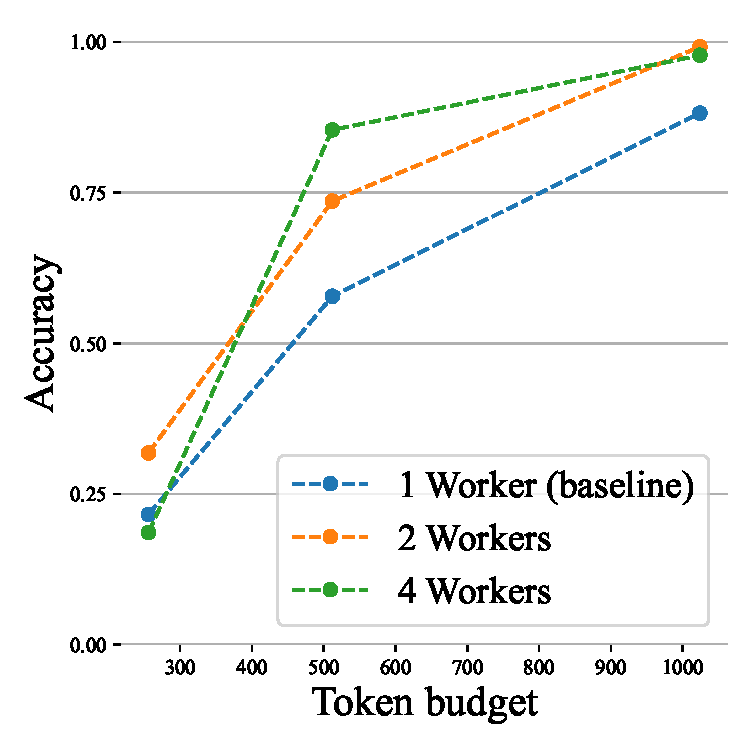
\includegraphics[width=0.4\textwidth]{resources/method_comparison_gsm8k.pdf}
  \end{center}
  \vspace{-10px}
  \caption{Evaluation results for synthetic problems with 5 GSM8k questions each.}\vspace{-10px}
  \label{fig:results_gsm8k}

\end{wrapfigure}


The results in Figure~\ref{fig:results_gsm8k} demonstrate that the parallel workers under Hogwild! Inference can indeed collaborate. When inspecting the generated traces, we found that the workers almost always spend the first few steps ``discussing'' how to split the work, then execute the assigned tasks. If one of the workers finishes their task early and there are no other tasks left, they typically either stall or double-check other workers' tasks. Note also that the accuracy with 4 workers is slightly higher than what can be extrapolated from 256 tokens per task. Upon closer examination, we found that many of the tasks require much fewer than 256 tokens, and when 4 workers attempt their tasks, the worker that finishes first often (but not always) takes up the remaining task. One anomalous result is when 4 workers have the budget of 256 tokens, where they underperform even the single worker baseline. This is because most of the budget is spent on coordination.

\textbf{LIMO tasks.} Next, we evaluate Hogwild! Inference on a more challenging problem set where there is no clear pattern of collaboration. We adopt the dataset from~\cite{ye2025limoreasoning} that contains mathematical problems that require thousands of tokens to solve reliably. Unlike our synthetic tasks, the problems in that dataset often do not have an obvious collaboration strategy ahead of time. However, as the LLM starts its reasoning chain, it often discovers situations where there are multiple cases or equations to solve in parallel, or alternatively, multiple possible strategies to solve a single problem. To evaluate on this dataset, we take 512 samples from the original dataset\footnote[11]{We used \url{https://huggingface.co/datasets/GAIR/LIMO}} (slightly over a half of the full dataset) and use the remaining samples for development.

Here, we compare the three Hogwild! cache layouts described in Section~\ref{sect:method_cache_layouts}. We also evaluate three baselines: i) a simple baseline that performs reasoning up to a given budget and is expected to provide the answer in \texttt{\textbackslash boxed\{ \}}. ii) an improved baseline where we prompt the LLM to produce the final answer if it did not generate one yet (same as above, \texttt{"Wait, given limited time ..."}, except \texttt{"5 answers"} $\longrightarrow$ \texttt{"the answer"}, generate at most 8 tokens) and iii) a naive parallel strategy inspired by~\cite{Wang2022SelfConsistencyIC}, where 2 workers both attempt to solve the task without communication, then we extract the answer with the same prompt as above.


We summarize our results in Figure~\ref{fig:results}: even in this more challenging task, Hogwild\! Inference with multiple workers can solve the problems faster than a single thread. Both interleaved cache and token-wise synchrony seem to contribute to the quality. Without interleaved cache (i.e. Contiguous layout), the workers seem to work well for smaller budgets, but their efficiency drops as they generate more tokens. We hypothesize that, when each worker generated many thousands of tokens, it becomes harder to notice and react to what the other assistant is doing. Conversely, interleaved layout without immediate synchronization performs poorly at small budgets, but then catches up as the workers are allowed to generate more tokens. We attribute this to the fact that, without step-wise synchrony, workers need more ``time'' to converge to a collaboration strategy. We present an illustrative example of the generation process for Hogwild! inference in Appendix~\ref{sect:appendix_examples}. We also report a more detailed accuracy breakdown for different budgets in Appendix~\ref{sect:appendix_extra_plots}.

Note, however, that these are only preliminary experiments that leave out many important questions: what is the impact of the prompting strategy? Does Hogwild!\! Inference work for other problem types (programming, function calling, etc)? Does the model's ability to reason on the problem correlate with how well it collaborates? Additionally, it is curious if we can \textit{train} the model to collaborate better through means such as supervised fine-tuning or reinforcement learning.

\begin{figure}[t]
    \centering
    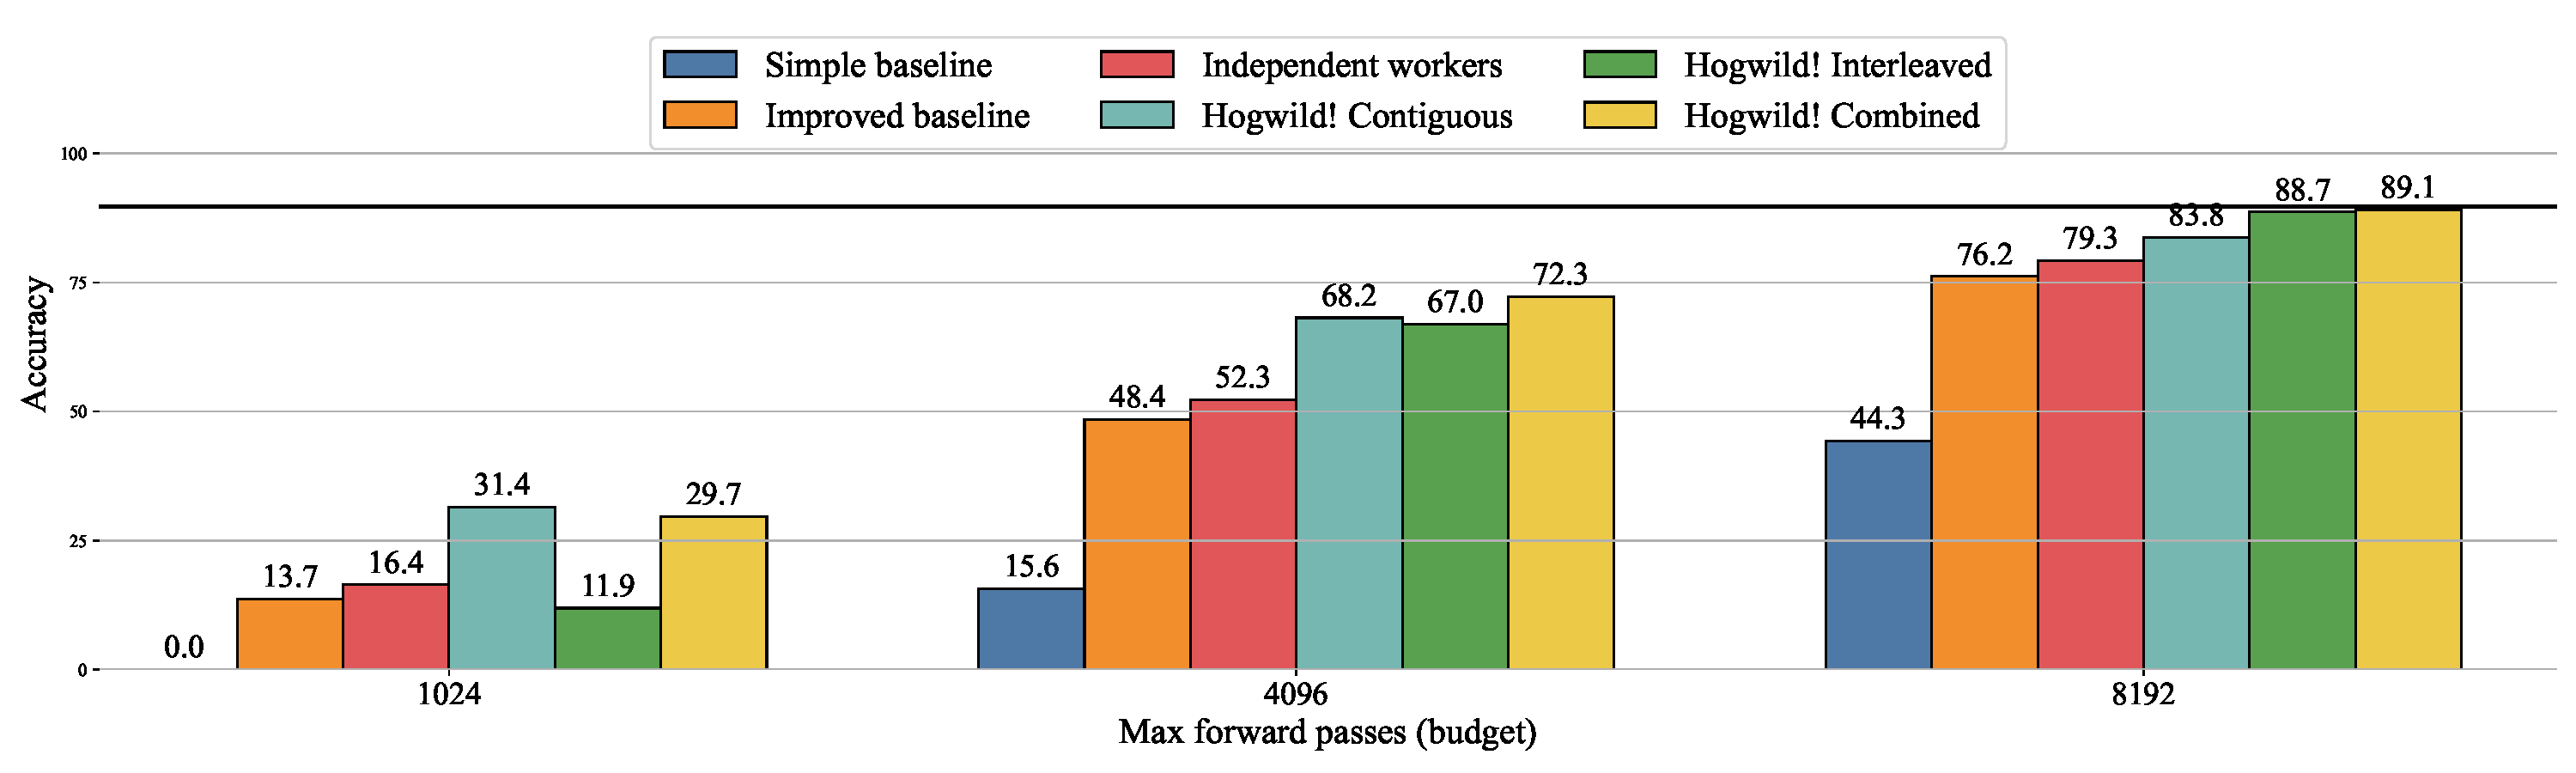
\includegraphics[width=1\linewidth]{resources/graphics.pdf}
    \caption{Evaluation on 512 LIMO tasks. The horizontal black line corresponds to running single-threaded reasoning for 16384 tokens (Accuracy 89.65\%). More budgets in Appendix~\ref{sect:appendix_extra_plots} (Figure~\ref{fig:limo_detailed_plot}).}
    \label{fig:results}
\end{figure}


